\section{Structure of an atom}
\begin{figure}
    \centering
    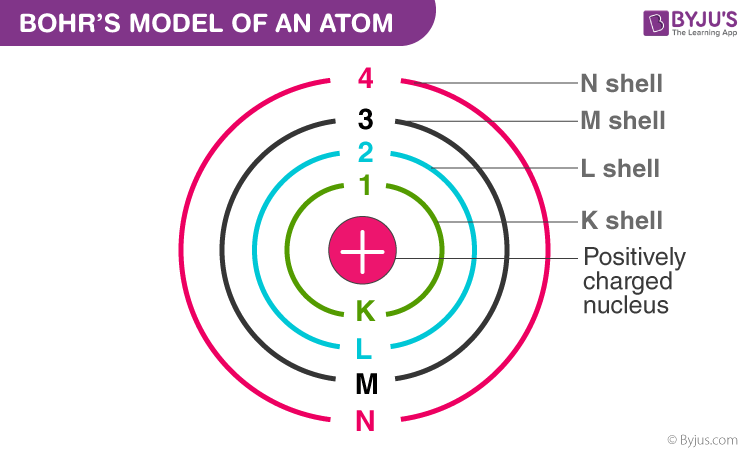
\includegraphics[width=0.75\linewidth]{atom.png}
    \caption{Structure of an atom}
\end{figure}
An atom of X element has Z number of protons, N number of neutrons [n(0)], and a mass (A) of Z+N. An element can be expressed as $\ch{^{A}_{Z}X}$ \par.
%-------------------------------------------------------------------------------------------------------------------------------------------------------------------------------------------------------------------------------------------------------------------------------------------------------------------------------------%
\section{Stability of atomic nuclei}
\begin{figure}
    \centering
    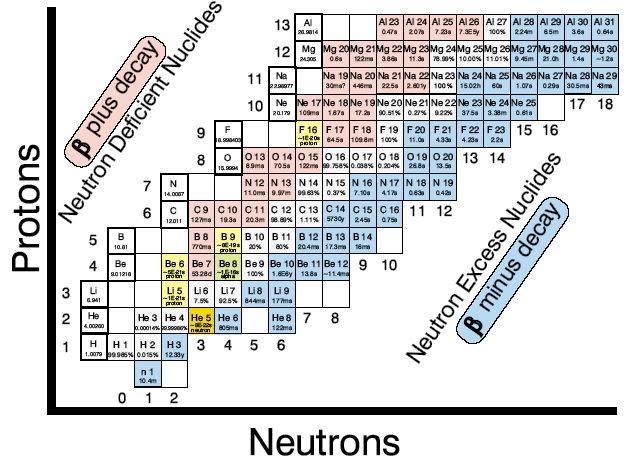
\includegraphics[width=0.75\linewidth]{chart_of_nucleides.png}
    \caption{Chart of Nucleides}
\end{figure}
%-------------------------------------------------------------------------------------------------------------------------------------------------------------------------------------------------------------------------------------------------------------------------------------------------------------------------------------%
\section{Radionucleides}
Some elements only exist as a radionucleide. Some elements exist with a very minute fraction of radioisotopes. There are also many artificial radionucleides.
%-------------------------------------------------------------------------------------------------------------------------------------------------------------------------------------------------------------------------------------------------------------------------------------------------------------------------------------%
\section{Activity and specific activity}
The nucleus of an unstable nucleide decays spontaneously to another nucleide (disintegration). Not affected by temperature, pressure, etc. Which nucleus will decay isn't predictable, but on average, it will decay. Activity is the decrease in radioactive nuclei per time.
\[A(t) := \frac{dN(t)}{dt}\]
The activity is expressed in Bq (1 disintegration per second). \\
Prefixes are used: k ($10^3$), M ($10^6$), G ($10^9$), T ($10^12$), m ($10^-3$), $\mu$ ($10^-6$), n ($10^-9$).
%-------------------------------------------------------------------------------------------------------------------------------------------------------------------------------------------------------------------------------------------------------------------------------------------------------------------------------------%
\section{Electromagnetic radiation}
Both a wave and a particle. The energy is expressed in J, or eV. $1\ eV = 1.6*10^{-19}\ J$. The binding energy of electrons on the outer shell is $\approx$ 30 eV. Photons and particles released are expressed in keV or MeV. X-rays are usually between 10 and 100 keV, while $\gamma$ radiation is usually between 100 and 1000 keV. 
%-------------------------------------------------------------------------------------------------------------------------------------------------------------------------------------------------------------------------------------------------------------------------------------------------------------------------------------%
\section{The radiation and the particles released during decay}
\subsection{$\alpha$ decay} Occurs when the nucleus is unstable, due to being too big. The parent atom $\ch{^{A}_{Z}X}$ gets split into a daughter atom $\ch{^{A-4}_{Z-2}Y}$ and an alpha particle $\ch{^{4}_{2}a}$.\\\\
\subsection{$\beta^{-}$ decay} Occurs when the nucleus is unstable, due to having an excess of neutrons. The parent atom $\ch{^{A}_{Z}X}$ gets split into a daughter atom $\ch{^{A}_{Z+1}Y}$, a beta particle $\ch{^{0}_{-1}e^{-}}$, and an anti-neutrino $\overline{v}_e$.\\\\
\subsection{$\beta^{+}$ decay} Occurs when the nucleus is unstable, due to having an excess of protons. The parent atom $\ch{^{A}_{Z}X}$ gets split into a daughter atom $\ch{^{A}_{Z+1}Y}$, a positron $\ch{^{0}_{+1}e^{+}}$, and a neutrino $v$. After a number of interactions, the positron $\beta{+}$ unites with an electron and converts its entire mass to energy. This annihilation produces 511 keV.\\\\
\subsection{Electron capture} The nucleus absorbs an electron from the electron cloud (usually from shell K -innermost). The parent atom $\ch{^{A}_{Z}X}$ absorbs an electron $\ch{^{0}_{-1}e^{-}}$, and gets split into a daughter atom $\ch{^{A}_{Z-1}Y}$, and a neutrino $v$.\\\\
\subsection{Gamma decay ($\gamma$)} Occurs when the atom is excited. The parent atom $\ch{^{A}_{Z}X*}$ gets excited and produces a daughter particle $\ch{^{A}_{Z}X}$ and a gamma ray $\gamma^{1}$. Internal conversion may occur (direct transfer of the energy of the nucleus to an electron).
\subsection{Internal conversion (IC)} Instead of $\gamma$ decay, internal conversion can occur. This is the the direct transfer of energy of the nucleus to an electron. The electron (conversion electron) is ejected from orbit with large energy, and can be detected as a $\beta^{-}$ particle, but with a sharply defined energy (unlike $\beta^{-}$, who share with neutrinos). Otherwise, can be considered a $\beta^{-}$ particle. This leaves a gap in the electron cloud, becoming unstable
\subsection{Follow-up processes: characteristic X-rays and Auger electrons} After the nucleus transfers energy to an electron or captures an electron, a vacancy is formed, filled by an electron a shell further away from the nucleus. The difference in binding energy causes the emission of characteristic X-ray spectrum (there's one emission per electron that descends = as many as electron shells there are). Due to this, other electrons may be ejected, known as Auger electrons.
%-------------------------------------------------------------------------------------------------------------------------------------------------------------------------------------------------------------------------------------------------------------------------------------------------------------------------------------%
\section{Parent-daughter relations}
After decay, the daughter nucleide may also be unstable. If the half-life is shorter, it's called ''ingrowth of activity'' (total activity grows). This must be taken into account.
%-------------------------------------------------------------------------------------------------------------------------------------------------------------------------------------------------------------------------------------------------------------------------------------------------------------------------------------%
\section{The time sequence in the decay processes}
An instable nucleide may have more than one decay process. Decay schemes explain graphically the decay. Parent level (top level), daughter level (bottom level), disintegration energy between them (Q). Increase in Z-value = right arrow; decrease in Z-value or EC = left arrow. 
